\documentclass[12pt, a4paper]{report}
\usepackage{amsmath, amssymb}
\usepackage{fancyhdr}
%\setlength{\headheight}{15pt}
\usepackage{geometry}
\usepackage{listings}
\geometry{margin=1.5in}
\usepackage[Rejne]{fncychap}
\pagestyle{fancy}
\usepackage{color}
\usepackage{blindtext}
\usepackage{import}
\usepackage{graphicx}
\usepackage{mathrsfs}
\usepackage{trfsigns}
\renewcommand{\chaptername}{Lecture}

\usepackage{import}
\usepackage{pdfpages}
\usepackage{transparent}
\usepackage{xcolor}

\setlength\parindent{0pt}

\newcommand\ddfrac[2]{\frac{\displaystyle #1}{\displaystyle #2}}

\newcommand{\incfig}[2][1]{%
  \def\svgwidth{#1\columnwidth}
  \import{figures}{#2.pdf_tex}
}

\pdfsuppresswarningpagegroup=1



\title{Energy Analytics}
\author{Adam Carrera}
\date{January 20, 2021}
\lhead{Week \thepart}

\begin{document}
  \maketitle
  \tableofcontents
  \part{Week 1}
  \chapter{Course Introduction}
  \section{Syllabus}
  The course syllabus is available on eLearning and coursebook. Professor and TA office hours are in MSTeams. Every Tuesday and Thursday 10 am - 11 am and 3 pm - 4 pm. Lectures will be posted Mondays and Wednesdays on MS Stream.

  \subsection{Homework}
  Homeworks are coding assingments that are submitted to elearning. Schedule is available in the syllabus.

  \subsection{Exams}
  The final exam will be open book. It will be assigned and submitted thorugh elearning.

  \subsection{Final Project}
  Recorded presentation and report through MS Teams and eLearning.

  \subsection{Course Description}
  Understand the basic concept of analytics, including descripting analytics and predictive analytics. Understand applications of analytics in energy industry. Know how to use mathematical software and other commercial packages. Know how to develop load, price, wind and solar forecasts.

  \section{Discussion}

  \subsection{Who makes up the most emissions?}

    China takes up the biggest share of global emissions at about 30\%. Electricity and heat make up 24.9\% of world greenhouse gas emissions (highest portion). There are several end uses for electricity and heat like buildings, refining, food. These processes create lots of $CO_2$. The majority of CO2 emissions in the US come from the Electricity sector, followed by transportation, and industry.

  \subsection{How do renewable technologies compare?}

    Renewable and carbon neutral technologies are utilized a lot less than coal and natural gas. Coal use has gone down from about 50\% of electricity generation in the US to 32.3\% (less than one third!). Natural gas however, has increased from 21.4\% to 32.3\%. Nuclear energy has remained constant throughout the years, due to the effrot required to build the plant. Hydropower has also remained constant through out the years. Other renewable sources are growing very fast (solar, wind power, biofuels, etc).

  \subsection{Wind and Solar Energy}

    Wind has the higest capactity of non-hydro renewables. By the end of 2018 the world was generating 591 Gigawatts of wind energy. Wind energy has also been growing very fast in the US as well. In Q3 2019 the US generated 100,128 MW, with Texas leading at ~27,000 MW. However in some parts of the US, the conditions are not suitable for wind turbines.

    PV (solar energy storage) has been steadily growing in the US as well. PV installations are split between Residential, Non-residential, and Utility. Solar energy resources vary with location as well.



  \subsection{What are the biggest drivers of renewable installations and penetration rates?}
    Policy is a big driver, states have different renewable portfolio standard targets. The costs to implement renewable energy has been decreasing over the years. Solar is a little more expensive than wind, but they are both becoming competitive with non-renewables. Utility-Scale PV costs have droped from \$5.52 per W to \$1.13 per W.

  \section{Renewables Integration}
    Power generation and energy consumption must be balanced. This balance becomes more challenging with renewables, because you cannot control how much wind blows or how much the sun shines.





  \part{Week 2}

  \chapter{Energy Analytics and R}

  \section{Energy Quiz}

  \begin{enumerate}
    \item How much of the energy in burning coal reaches the consumer as electricity? (33\%)
    \item Which State consumes the most energy? (Texas)
    \item Which state produces the most coal? (Wyoming)
    \item What country produces the most coal? (China)
    \item Which country generates the most electricity from nuclear power? (United States)
    \item What country generates the greatest share of its electricity from wind power? (Denmark)
    \item Electricity is called a secondary energy source because ... (We get it from converting other energy sources)
    \item Most of the energy we use originally came from? (The sun)
  \end{enumerate}

  \section{Power System Background}

  Power systems have transitioned from centralized to distributed generation (Solar panels on roofs, batteries, PV panels, small generators). One challenge is that the energy flows in two directions, instead of one. Another challenge is that renewable energy is variable and uncertain. However, advanced communication has allowed decentralized control of devices.

  \subsection{Power System Operations Timescales}

  The power system load changes throughout the day. As your load changes, your power generation should change as well. Regulation is seconds to minutes, load flowing is minutes to hours, and scheduling is the entire day. Unit commitment refers to several day.

  \subsection{Energy Sector}

  Electricity is only one part of the energy sector. There is a trade off between fixed costs and operating costs.
  \begin{itemize}
    \item Nuclear and Solar have high fixed cost, low operating costs
    \item Natural gas/oil have low fixed costs, high operating costs (depends on fuel prices)
    \item Coal, wind, hydro are in between
  \end{itemize}

  \noindent
  A units \textbf{Capacity Factor} is important to determining ultimate cost of electricity. Wind has a low capacity factor (50\%). Some renewables have tax credits, which affect the economics. Different renewables have different levelized costs (USD/kwH). The levelized cost of Solar PV has decreased from 2010 to 2014.

  \newpage

  \subsection{Conventional Power System}

  The conventional power system is a one way system. You generate the power and send it to the customer. In later lectures we will talk about different changes in power systems to centralized systems to decentralized systems.
  \begin{enumerate}
    \item Generation (Source)
    \item Transmission Substation (Change voltage to a suitable value)
    \item Transmission System (Carry energy long distances)
    \item Distribution Substation (Change volatge, smaller than transmission substation)
    \item Distribution System (Power lines, distribute to customer)
    \item Customer (Loads)
  \end{enumerate}

  \subsection{Power Plant Classification}

  There are 3 categories.

  \begin{enumerate}
    \item Base-Load Generating Units
    \begin{itemize}
      \item Constant power generation over time
      \item Long start-up and shut-down times
      \item Low cost of production, but high capital investment
      \item ex. Nuclear, Hydroelectric, High-Performance Steam Turbine Plant
    \end{itemize}
    \item Intermediate (Load Following) Generating Plant
    \begin{itemize}
      \item Typicall runs at full-load between 2,000 - 5,000 hrs/yr
      \item Operation and economic characteristics somewhere betwwen base-load and peak-load
      \item ex. Simple Steam Turbine Plant, Old Base-Load Plant, combined Gase and Steam Turbine Plant, Sleected Hydroelectric Power Plant
    \end{itemize}
    \item Peak-Load Generating Units
    \begin{itemize}
      \item Quick starting and shutdown capability
      \item Runs between 100 - 2,500 hrs/yr during peak loads
      \item Standby and emergency units
      \item ex. Gas Turbine, Diesel Engine, Hydro - Pumped Storage
    \end{itemize}
  \end{enumerate}

  \subsection{Interconnections}

  The US has 3 synchronous grids (interconnections). The Eastern Interconnection, Western Interconnnection, Texas Interconnection (cool!).

  \subsection{Renewable Energy and Distributed Generation}

  Most renewable energy will be converted into electricity. The resource will be distributed geographically and mostly dependent on changing weather and climate. However, the resource cannot be directly controlled in the manner of conventional generation (variable and uncertain output).

  Renewable resources are more distributed than conventional types. They are often connected at low voltages. Increasing the input from renewable energy sources requires a revision of the way power systems are designed and operated in order to better accomodate these sources better.

  \section{Analysis}

  \subsection{Actionable Decision Support \& Automation}

  The amount of analytics and human input depends on the type of analysis. Our goal is to use prescriptive analytics, so the computer will either support a decision, or make the decision automatically.

  \begin{itemize}
    \item Descriptive - What happened?
    \item Diagnostic - Why did it happen?
    \item Predictive - What will happen?
    \item Prescriptive - What should I do?
  \end{itemize}

  \subsection{Behind the Meter (BTM) Solar Forecasting}
  Different levels of difficulty associated with solar forecasting. BTM is for very small systems.
  \begin{itemize}
    \item Bottom-up approach
    \item Multi-timescale Forecasting
    \item Distributed Solar Ramp forecasting
  \end{itemize}

  \subsection{Types of Load Forecasting}

  \begin{itemize}
    \item Short term forecasts (one hour to a week)
    \item Medium forecasts (a month up to a year)
    \item Long term forecasts (over one year)
  \end{itemize}

  \subsection{Key Methods}

  \begin{itemize}
    \item Time series models, visualization, regression models, decomposition
    \item Machine Learning models
    \item Deep learning models
    \item Probablility, distribution, visualization
  \end{itemize}

  \section{Distributions}

  We will talk about probability distributions more in-depth in the future.

  \subsection{Normal Distribution}

  \begin{itemize}
    \item Probability density function
    \item Cumulative distribution function
  \end{itemize}


  \chapter{R in Class}

  \part{Week 3}

  \chapter{Conventional Power Generation}

  \section{Thermal Power Generation}

  \begin{itemize}
    \item Coal-fired thermal power: Baseload operation
    \item LNG-fired thermal power: Base to middle load operation (Liquid Natural Gas)
    \item Oil-fired thermal power: Middle to peak load operation
  \end{itemize}

  The basic principle is,

  \begin{itemize}
    \item Fuel tank sends fuel to boiler
    \item Boiler boils water which creates team
    \item Turbine is driven by the high temperature steam
    \item Generator is powered by the turbine
  \end{itemize}

  \subsection{Coal Generation Details}

  Coal plants are divided into Regular, Super Critical, and Ultra Super Critical plants. The pressure levels, efficiency levels, and temperature increase with each plant.

  \subsection{Grid Integration Details}

  Coal plants are base load, which means long start up and shutdown times (24 hrs or more!). The long minimum run times and high minimum generation levels are a challenge for integration.

  \subsection{Plant Scherer - Georgia}

  \begin{itemize}
    \item Total Capacity: 3,520 MW
    \item Largest GHG emitter in the US (20M tons per year)
    \item 7th largest plant in the US (by Capacity)
    \item Capacity Factor: 61.2 \%
    \item Consumes 11M tons of coal per year
    \item Each of four cooling towers circulates 270k gallons of water per minutes with 8k gallons lost to evaporation
  \end{itemize}

  \section{Discussion}

  \begin{itemize}
    \item What are the three largest generation plants in the US?
    \item What technologies would you expect them to be?
  \end{itemize}

  See Table \ref{tab:4.1}.

  \begin{table}
    \centering
    \begin{tabular}{c c}
      Plant Name & Energy Source \\
      \hline
      Grand Coulee & Hydroelectric \\
      Palo Verde & Nuclear \\
      Martin & Natural gas, fuel oil
    \end{tabular}
    \caption{Largest US Power Plants and Primary Energy Source}
    \label{tab:4.1}
  \end{table}

  \section{Natrual Gas Plants}

  Conversion efficiencies typically between 20 - 35\% with temperatures of 2000 F. These turbines can generally start up and shut down faster, as well as being able to ramp up more quickly. May be flexible with fuel oil as an alternative.

  \subsection{Turbine Types}

  \begin{itemize}
    \item Heavy Frame
      \begin{itemize}
        \item Lower pressure ratio ($ < $ 20)
        \item Tend to be larger
      \end{itemize}
    \item Aero-derivative
      \begin{itemize}
        \item Higher pressure ratio ($ > $ 30)
        \item Tend to be smaller
      \end{itemize}
  \end{itemize}

  \section{Discussion}

  Gas and steam turbines have low efficiencies. How can we increase that efficiency?

  \begin{itemize}
    \item We can combine the gas and steam turbines, this is called a combined cycle.
    \item Another way is to have the gas from the gas plant boil the water for the steam plant.
  \end{itemize}

  The efficiency can be increase to about 50 - 60\%. Can be operated seperately as well. The typical start-up time for (older) full units is 2-4 hours. These are historically mid range units.

  \section{Nuclear Generators}

  Nuclear is a carbon neutral technology.

  \begin{itemize}
    \item Containment building holds the reactor, which boils the water
    \item The steam powers the turbine, generating electricity
  \end{itemize}

  \subsection{Nuclear Facts}

  \begin{itemize}
    \item Over 400 plants in 30 countries
    \item Power form Fission, not fusion
    \item Uses uranium 235
    \item Nuclear waste disposal is still an unsolved problem
  \end{itemize}

  \subsection{Grid Integration}

  \begin{itemize}
    \item Base load, week long startup and shutdown times
    \item Very little ramping capability
    \item Large capacity plants
    \item Ultra-high minimum generation levels, often 90\% capacity
  \end{itemize}

  \section{Hydropower}

  \begin{itemize}
    \item Conventional - dams
    \item Unconventional hydropower
      \begin{itemize}
        \item Hydrokinetic power
      \end{itemize}
  \end{itemize}

  Which country produced the most hydropower?

  \begin{enumerate}
    \item China
    \item Brazil
    \item Canada
    \item US
    \item Russia
  \end{enumerate}


  We are unlikely to build more conventional hydro any more (environment concerns). But we can still build pumped storage. Here are some more facts.

  \begin{itemize}
    \item 80 - 90\% efficiency
    \item 6 - 10 \% of US electricity generation
    \item Roughly 100 GW of capacity
    \item 80k dams in the US, 2.4k have hydropower
    \item about 20\% of world electricity usage
    \item 77\% of Brazilian power
    \item about 17\% of Chinese power
    \item 95\% of power in Norway
  \end{itemize}

  \section{Discussion}


  What are some of the limitations towards expanding hydropower in the US? Internationally?

  \section{Geothermal Generation}

  Cold water is pumped down to the earth. The heat of the earth heats up the water making steam, which travels up to the generating station.

  \begin{itemize}
    \item Dry steam (150 C)
    \item Flas steam (180 C)
    \item Binary Cycle (60 C)
  \end{itemize}






  \chapter{Probability \& Distribution}

  \section{Probability Density Function (PDF)}

  Suppose we have some variable $ X \sim f(x) $ where $ f(x) $ is the probability density function (pdf) of $ X. $

  The requirements on $ f(x) $ are:

  \begin{itemize}
    \item $ f(x) \geq 0  \quad \forall x \in X. $ Where $ X $ is the domain of $ X. $
    \item $ \int f(x)dx = 1. $
  \end{itemize}

  The normal distribution pdf has the form,

  \[
      f(x) = \ddfrac{1}{\sigma \sqrt{2\pi}}e^{- \ddfrac{(x - \mu)^2}{2\sigma ^2}}
    .\]

  \newpage
  \section{Standard Normal Distribution}

  If $ X \sim N(0, 1), $ then $ X $ follows a normal distribution.

  \begin{equation}
    f(x) = \ddfrac{1}{\sqrt{2\pi}}e^{- \ddfrac{x ^2}{2}}
  \end{equation}

  \begin{figure}
    \centering
    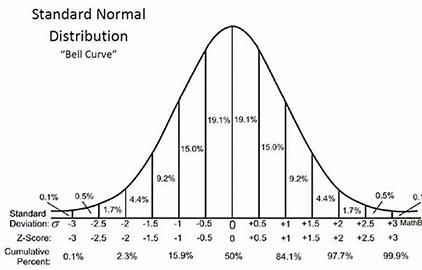
\includegraphics{figures/normaldis.jpg}
    \caption{Standard Normal Distribution}
  \end{figure}

  \section{Cumulative Distribution Function (CDF)}

  The CDF $ F(x) $ for a discrete random variable $ X $ gives, for any specified number $ x $ the probability $ P(X \leq x). $ Obtained by summing the pdf $ p(y) $ over all possible values $ y $ s.t $ y \leq x. $ The CDF of a continuous random variable gives the same probabilities $ P(X \leq x) $ and is obtained by integrating the pdf $ f(y) $ between minus infinity and x.

  \begin{equation}
    F(x) = P(X \leq x) = \int_{\infty}^{\infty} f(y)dy
  \end{equation}

  For each x, F(x) is the area under the density curve to the left of x.

  \begin{figure}
    \centering
    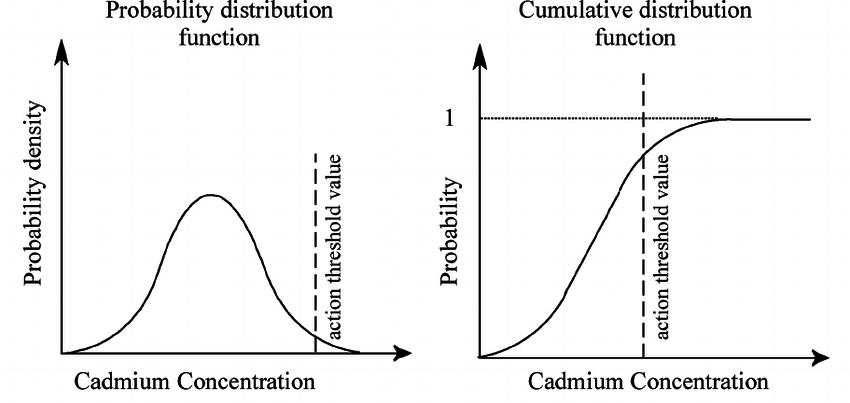
\includegraphics[width=\textwidth]{figures/cumulativedist.png}
    \caption{A PDF and associated CDF}
  \end{figure}

  \subsection{Obtaining PDF from CDF}

  If X is a continuous random variable with pdf $ f(x) $ and cdf $ F(x) $, then at every $ x $ at which the derivative $ F'(x) $ exists,

  \[
      F'(x) = f(x)
    .\]

  \begin{table}
    \centering
    \caption{Properties of Normal Distribution}
    \begin{tabular}{c c}
      PDF & see above section \\
      CDF & $ \frac{1}{2} \left( 1 + erf \left( \frac{x - \mu}{\sigma\sqrt{2}} \right) \right). $ \\
      Quantile & $ \mu + \sigma\sqrt{2}erf^-1 (2F - 1). $ \\
      Mean & $ \mu. $ \\
      Median & $ \mu. $ \\
      Mode & $ \mu. $ \\
      Variance & $ \sigma ^2. $
    \end{tabular}

  \end{table}


  \section{Gamma Distribution}

  PDF:

  \begin{equation}
    f(x;k,\theta) = \ddfrac{x^{k-1}e^{-\ddfrac{x}{\theta}}}{\theta^k \Gamma(k)}, \quad x, k, \theta > 0
  \end{equation}

  CDF:

  \begin{equation}
    F(x;k,\theta) = \int_{0}^{x} f(u;k,\theta)du = \frac{\gamma \left( k, \frac{x}{\theta} \right)}{\Gamma(k)}
  \end{equation}

  where k is the shape parameter, and $ \theta $ is the scale parameter.

  \begin{figure}
    \centering
    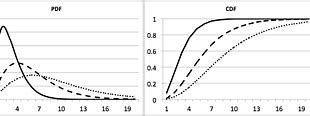
\includegraphics{figures/gamma}
    \caption{Gamma PDF and CDF}
  \end{figure}

  \section{Weibull Distribution}

  \begin{figure}
    \centering
    \normalsize
    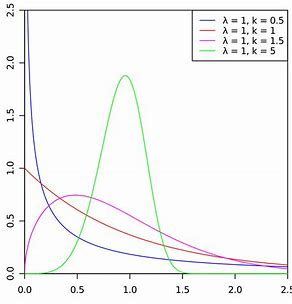
\includegraphics[width=0.5\textwidth]{figures/weibull}
    \caption{Weibull PDF}
  \end{figure}

  \section{Problem of Estimation}

  We want to estimate $ f(x) $ or $ F(x) $ from a smaple of data $ \{x_j\}_{j=1}^n. $

  Different approaches

  \begin{enumerate}
    \item Histogram estimates
    \item Kernel density estimates
    \item Single distribution estimates
  \end{enumerate}

  \section{Single Distribution Estimates}

  Use R package: fitdistrplus. KDE with Gaussian kernel

  \part{Week 4}

  \chapter{Wind Energy Analytics}

  \section{Wind Map Information}

  \begin{itemize}
    \item Wind map is digitized using image processing tools
    \item Total area under different average wind speeds (AWS) is estimated with an interval of 0.5 m/s
    \item A normal distribution is fitted to represent the geographical distribution of average wind speeds over contiguous USA
  \end{itemize}

  \[
      \mu = 5.6 \text{ m/s}, \quad \sigma = 1.3 \text{ m/s}
    .\]

  \section{Discussion}

  What are the five largest wind turbine manufacturers in terms of global market share?

  \begin{itemize}
    \item Goldwind
    \item Vestas
    \item GE Wind
    \item Siemens
    \item Gamesa
  \end{itemize}

  \section{Wind Generator Types}

  \begin{itemize}
    \item Type 1 - Fixed-speed wind turbine
    \item Type 2 - Variable-slip wind turbine
    \item Type 3 - Pitch controlled wind rotor
    \item Type 4 - Full converter wind turbine
  \end{itemize}

  Type 1 has a squirell cage induction generator, type two has a wound rotor induction generator and a control signal.

  \section{Offshore Pros and Cons}

  Advantages

  \begin{itemize}
    \item Generally higher capacity factors
    \item Less visual impact
    \item Often closer to load centers
    \item Better correlation with load in some locations
  \end{itemize}

  Disadvantages

  \begin{itemize}
    \item Higher installation costs
    \item Maintenance issues
  \end{itemize}







  \part{Week 5}

  \chapter{Turbulence}

  \section{Wind Energy - Turbulence}

  Wake loss leads to significant energy loss, about 5 to 20 percent from the whole plant. Turbulence is characterized by ambient and wake turbulence.

  \begin{itemize}
    \item ambient turbulence - normal turbulence at the site that weould be experienced by one turbine
    \item wake turublence - caused by upwind turbines shading those downstream
  \end{itemize}

  How do the turbulence conditions affect wind power differently?

  \subsection{Monitoring Data}

  Using Xcel Cedar Creek wind plant data, we can

  \begin{itemize}
    \item determine data sets for in and out of wake
    \item construct surrogate models $ P = f(U), P = f(U, TI). $ (TI - Turbulence Intensity)
    \item Quantify the uncertainty in turbine power generation
  \end{itemize}

  \subsection{In and Out of Wake Scenarios}

  Pick one turbine and calculate which turbines are in its wake based on wind direction.

  \subsection{Surrogate Modeling: In-Wake and Out-of-Wake Scenarios}

  For each set of data, two surrogate models were developed to represent the turbine power generation. As a function of wind speed and as a function of both wind speed and turbulence intensity.

  The turbulence intensity is defined as the standard deviation of the wind speed within a short time period divided by the mean wind speed during that time period.

  \begin{equation}
    TI = \frac{\sigma_U}{U}
  \end{equation}

  \subsection{Support Vector Regression}

  Surrogate modeling is concerned with the construction of approximation models to estimate system performance and to develop relationships between specific system inputs and outputs.

  \subsection{Uncertainty in the Power Response}

  Once we have our models we can quantify uncertainty.

  The discrepancy between the actual power generation and the power curve estimation of a wind turbine can be attributed to the following major factors:

  \begin{itemize}
    \item Wind shear - the variation of wind with vertical distance from the ground
    \item Turbulence effects - the power generation depends on both mean wind speed and turbulence
    \item Turbine reliability - the uncertainty in the turbine performance
  \end{itemize}

  We want to illustrate how the uncertainty is different between in and out of wake scenarios. This is measured by the uncertainty with respect to the reported power curve

  \begin{equation}
    E_{pc} = P_c(U) - P_g(U)
  \end{equation}

  Where Pc is expected power and Pg is recorded power. Epc is the error of power curve. If we wanted to estimate based on only wind speed we would have. The uncertainty in power generation with respect to estimated power response that only accounts for mean wind speed. \textbf{These are both error distributions.}

  \begin{equation}
    E_{pf} = P_g(U) - P_f(U)
  \end{equation}

  Where Pf is the surrogate estimation. Finally, we









\end{document}
